\documentclass[10pt]{article}
\usepackage[a4paper,margin=18mm]{geometry}
\usepackage{amsmath,amssymb,booktabs,array,enumitem}
\usepackage[T1]{fontenc}\usepackage{lmodern}
\usepackage{tikz}\usetikzlibrary{shapes.gates.logic.US,positioning,arrows.meta,patterns,calc}
\usepackage[hidelinks]{hyperref}
\setlength{\parindent}{0pt}\setlength{\parskip}{4pt}
\setlength{\emergencystretch}{2em}
\newcommand{\VDD}{V_{DD}}
\newcommand{\mos}[4]{\begin{scope}[shift={(#1,#2)}]
\draw (0,.24)--(0,-.24);\draw (0,.20)--(.25,.20)--(.25,.5);
\draw (0,-.20)--(.25,-.20)--(.25,-.5);\draw (-.16,.23)--(-.16,-.23);
\ifnum#4=1\draw (-.26,0) circle (.06);\draw (-.75,0)--(-.32,0);\else\draw (-.75,0)--(-.16,0);\fi
\node[anchor=east,font=\scriptsize] at (-.76,0) {$#3$};\end{scope}}
\newcommand{\ground}[2]{\draw (#1,#2)--(#1,{#2-.12});\draw ({#1-.17},{#2-.12})--({#1+.17},{#2-.12});\draw ({#1-.11},{#2-.20})--({#1+.11},{#2-.20});}
\newcommand{\rail}[3]{\draw (#1,#2)--(#1,{#2+.14});\node[above,font=\scriptsize] at (#1,{#2+.14}) {$#3$};}

\newcommand{\hmos}[4]{\begin{scope}[shift={(#1,#2)}]
\draw(-.24,0)--(.24,0);\draw(-.2,0)--(-.2,-.25)--(-.5,-.25);\draw(.2,0)--(.2,-.25)--(.5,-.25);
\draw(-.23,.16)--(.23,.16);
\ifnum#4=1\draw(0,.26)circle(.06);\draw(0,.32)--(0,.75);\else\draw(0,.16)--(0,.75);\fi
\node[below,font=\scriptsize]at(0,-.32){#3};\end{scope}}
% Independently traced from the printed Fall 2007 Q3 symbolic layout.
% Inline these macros into standalone documents; geometry is normalized.
\newcommand{\OriginalLayout}{%
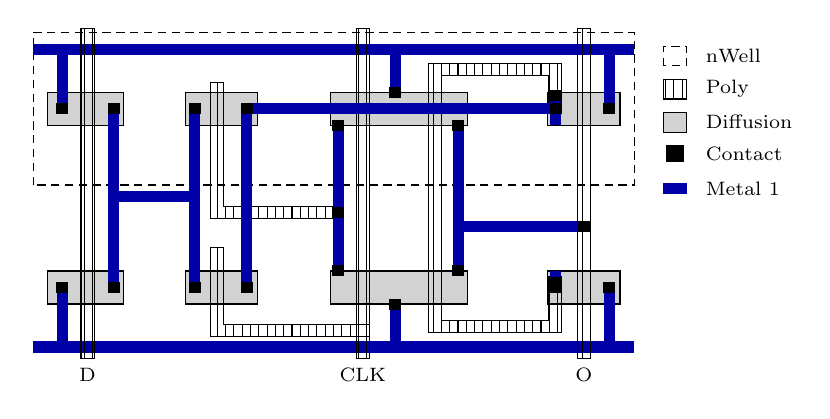
\begin{tikzpicture}[x=.92cm,y=.84cm,font=\scriptsize,
  act/.style={fill=gray!35,draw=black,thin},
  poly/.style={draw=black,fill=white,pattern=vertical lines,pattern color=black},
  metal/.style={draw=blue!65!black,line width=4pt},
  ct/.style={fill=black,draw=black}]
% Printed n-well, metal rails and four diffusion islands in each row.
\draw[densely dashed](-.05,2.65)rectangle(8.25,4.95);
\draw[metal](-.05,4.7)--(8.25,4.7);
\draw[metal](-.05,.2)--(8.25,.2);
\foreach \y in {3.8,1.1}{
 \path[act](.15,{\y-.25})rectangle(1.2,{\y+.25});
 \path[act](2.05,{\y-.25})rectangle(3.05,{\y+.25});
 \path[act](4.05,{\y-.25})rectangle(5.95,{\y+.25});
 \path[act](7.05,{\y-.25})rectangle(8.05,{\y+.25});}
% Continuous external D/CLK/O gates; the TG clock gate is split.
\foreach \x in {.7,4.5,7.55}{\path[poly]({\x-.09},.03)rectangle({\x+.09},5.02);}
\path[poly](2.4,2.14)--(4.16,2.14)--(4.16,2.32)--(2.58,2.32)--(2.58,4.2)--(2.4,4.2)--cycle;
\path[poly](2.4,.36)--(4.59,.36)--(4.59,.54)--(2.58,.54)--(2.58,1.7)--(2.4,1.7)--cycle;
% Continuous storage-inverter poly, with both U-return arms.
\path[poly](5.41,.42)--(7.24,.42)--(7.24,1.27)--(7.06,1.27)--(7.06,.60)--(5.59,.60)--(5.59,4.30)--(7.06,4.30)--(7.06,3.90)--(7.24,3.90)--(7.24,4.48)--(5.41,4.48)--cycle;
% Supply contacts (a metal crossing alone is not an electrical contact).
\draw[metal](.35,3.8)--(.35,4.7);
\draw[metal](.35,1.1)--(.35,.2);
\draw[metal](4.95,4.05)--(4.95,4.7);
\draw[metal](4.95,.85)--(4.95,.2);
\draw[metal](7.9,3.8)--(7.9,4.7);
\draw[metal](7.9,1.1)--(7.9,.2);
% dbar: first-inverter drains and left TG terminals.
\draw[metal](1.06,3.8)--(1.06,1.1);
\draw[metal](1.06,2.48)--(2.18,2.48);
\draw[metal](2.18,3.8)--(2.18,1.1);
% u: TG right terminals, final-inverter drains and U-poly contacts.
\draw[metal](2.9,3.8)--(2.9,1.1);
\draw[metal](2.9,3.8)--(7.16,3.8);
% Separate final-drain stubs: their common u connection is via the U-poly.
% A vertical Metal1 through the middle gap would wrongly short the O route.
\draw[metal](7.16,4.0)--(7.16,3.55);
\draw[metal](7.16,1.35)--(7.16,1.1);
% CLKB: CLK inverter drains return to the UPPER TG poly only.
\draw[metal](4.16,3.55)--(4.16,1.35);
% O: storage-inverter drains join the final O poly at one contact.
\draw[metal](5.82,3.55)--(5.82,1.35);
\draw[metal](5.82,2.02)--(7.55,2.02);
\foreach \x/\y in {.35/3.8,.35/1.1,1.06/3.8,1.06/1.1,2.18/3.8,2.18/1.1,2.9/3.8,2.9/1.1,4.16/3.55,4.16/1.35,4.95/4.05,4.95/.85,5.82/3.55,5.82/1.35,7.16/3.8,7.16/1.1,7.9/3.8,7.9/1.1,4.16/2.23,7.16/4.0,7.16/1.18,7.55/2.02}{
 \path[ct]({\x-.075},{\y-.075})rectangle({\x+.075},{\y+.075});}
\node[below]at(.7,.02){D};\node[below]at(4.5,.02){CLK};\node[below]at(7.55,.02){O};
\draw[densely dashed](8.65,4.45)rectangle(8.97,4.75);\node[right]at(9.10,4.6){nWell};
\path[poly](8.65,3.95)rectangle(8.97,4.25);\node[right]at(9.10,4.1){Poly};
\path[act](8.65,3.45)rectangle(8.97,3.75);\node[right]at(9.10,3.6){Diffusion};
\path[ct](8.69,3.0)rectangle(8.93,3.24);\node[right]at(9.10,3.12){Contact};
\draw[metal](8.65,2.6)--(8.97,2.6);\node[right]at(9.10,2.6){Metal 1};
\end{tikzpicture}}

\newcommand{\SolutionLayout}{%
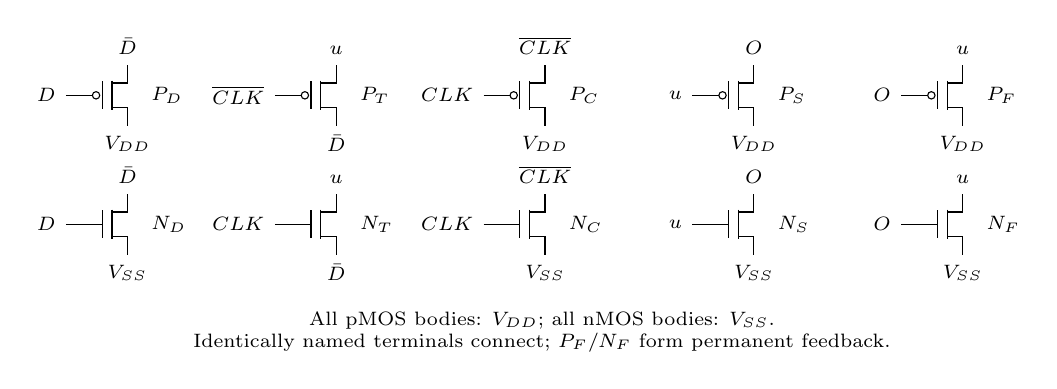
\begin{tikzpicture}[scale=.78,font=\scriptsize]
% Every MOS is explicit. Identically named terminals are joined.
\mos{0}{1}{D}{1}\node[right]at(.48,1){$P_D$};\node[above]at(.25,1.5){$\bar D$};\node[below]at(.25,.5){$V_{DD}$};
\mos{3.4}{1}{\overline{CLK}}{1}\node[right]at(3.88,1){$P_T$};\node[above]at(3.65,1.5){$u$};\node[below]at(3.65,.5){$\bar D$};
\mos{6.8}{1}{CLK}{1}\node[right]at(7.28,1){$P_C$};\node[above]at(7.05,1.5){$\overline{CLK}$};\node[below]at(7.05,.5){$V_{DD}$};
\mos{10.2}{1}{u}{1}\node[right]at(10.68,1){$P_S$};\node[above]at(10.45,1.5){$O$};\node[below]at(10.45,.5){$V_{DD}$};
\mos{13.6}{1}{O}{1}\node[right]at(14.08,1){$P_F$};\node[above]at(13.85,1.5){$u$};\node[below]at(13.85,.5){$V_{DD}$};
\mos{0}{-1.1}{D}{0}\node[right]at(.48,-1.1){$N_D$};\node[above]at(.25,-.6){$\bar D$};\node[below]at(.25,-1.6){$V_{SS}$};
\mos{3.4}{-1.1}{CLK}{0}\node[right]at(3.88,-1.1){$N_T$};\node[above]at(3.65,-.6){$u$};\node[below]at(3.65,-1.6){$\bar D$};
\mos{6.8}{-1.1}{CLK}{0}\node[right]at(7.28,-1.1){$N_C$};\node[above]at(7.05,-.6){$\overline{CLK}$};\node[below]at(7.05,-1.6){$V_{SS}$};
\mos{10.2}{-1.1}{u}{0}\node[right]at(10.68,-1.1){$N_S$};\node[above]at(10.45,-.6){$O$};\node[below]at(10.45,-1.6){$V_{SS}$};
\mos{13.6}{-1.1}{O}{0}\node[right]at(14.08,-1.1){$N_F$};\node[above]at(13.85,-.6){$u$};\node[below]at(13.85,-1.6){$V_{SS}$};
\node[align=center]at(7,-2.85){All pMOS bodies: $V_{DD}$; all nMOS bodies: $V_{SS}$.\\Identically named terminals connect; $P_F/N_F$ form permanent feedback.};
\end{tikzpicture}}

\begin{document}
\begin{center}{\large\bfseries EE3032 Introduction to VLSI Design -- Final}\\Fall 2007\end{center}
\textbf{1. (26\%)} Answer the following problems.
\begin{enumerate}[label=(\alph*),leftmargin=7mm,itemsep=2pt]
\item List major steps of the full-custom design flow. (8\%)
\item List two basic rules for drawing the layout of a standard cell. (4\%)
\item List two major problems of dynamic logic. (4\%)
\item List two limitations of CMOS domino logic. (4\%)
\item What are core-limited design and pad-limited design? (6\%)
\end{enumerate}
\textbf{2. (10\%)} What logic function does the circuit of Figure 1 realize? Explain your answer in detail.
\begin{center}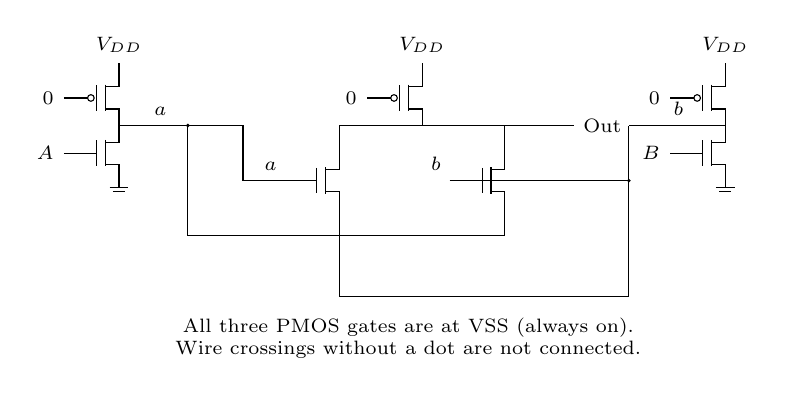
\begin{tikzpicture}[scale=.7,font=\scriptsize]
\mos{0}{5}{0}{1}\rail{.25}{5.5}{V_{DD}}\mos{0}{4}{A}{0}\ground{.25}{3.5}\node[above]at(1,4.5){$a$};\draw(.25,4.5)--(1.5,4.5);
\mos{11}{5}{0}{1}\rail{11.25}{5.5}{V_{DD}}\mos{11}{4}{B}{0}\ground{11.25}{3.5}\node[above]at(10.4,4.5){$b$};\draw(11.25,4.5)--(9.5,4.5);
\mos{5.5}{5}{0}{1}\rail{5.75}{5.5}{V_{DD}}\draw(4.25,4.5)--(8.5,4.5)node[right]{Out};\mos{4}{3.5}{\phantom{a}}{0}\mos{7}{3.5}{\phantom{b}}{0}\draw(4.25,4)--(4.25,4.5);\draw(7.25,4)--(7.25,4.5);\node[above]at(3,3.5){$a$};\node[above]at(6,3.5){$b$};
\draw(1.5,4.5)--(2.5,4.5)--(2.5,3.5)--(3.25,3.5);\draw(1.5,4.5)--(1.5,2.5)--(7.25,2.5)--(7.25,3);\fill(1.5,4.5)circle(1pt);
\draw(4.25,3)--(4.25,1.4)--(9.5,1.4)--(9.5,4.5);\draw(9.5,3.5)--(6.25,3.5);\fill(9.5,3.5)circle(1pt);
\node[align=center]at(5.5,.65){All three PMOS gates are at VSS (always on).\\Wire crossings without a dot are not connected.};\end{tikzpicture}\\Figure 1: A logic circuit. Added labels $a,b$ identify the intermediate nodes.\end{center}
\textbf{3. (14\%)} Figure 2 shows a layout view of a CMOS circuit. Draw its transistor schematic diagram.
\begin{center}\OriginalLayout\\Figure 2: Symbolic layout of a CMOS circuit. Geometry normalized; contacts and split poly preserved.\end{center}
\newpage
\textbf{4. (20\%)} The circuit in Figure 3 implements a high-speed one-bit full adder. Complete the following problems.
\begin{enumerate}[label=(\alph*),leftmargin=7mm]
\item What type of logic was used to implement this circuit? (5\%)
\item Describe the operation of the circuit. (5\%)
\item The drain and gate capacitances of PMOS and NMOS are 0.2 fF and 1 fF, respectively. The leakage current of output nodes $\bar C_{n+1}$ and $\bar S_n$ is 1 nA. Also $V_{DD}=1.8$ V and the inverter switching threshold is $V_{DD}/2$. Determine the lowest operating speed of the circuit. (10\%)
\end{enumerate}
\begin{center}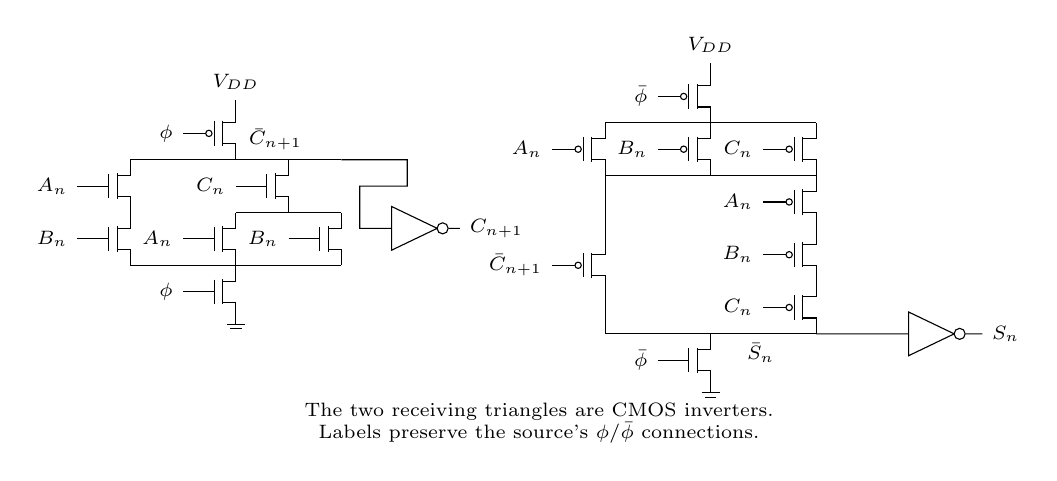
\begin{tikzpicture}[scale=.67,font=\scriptsize]
\mos{2}{5.8}{\phi}{1}\rail{2.25}{6.3}{V_{DD}}\draw(.25,5.3)--(4.25,5.3);\node[above]at(3,5.3){$\bar C_{n+1}$};\mos{0}{4.8}{A_n}{0}\mos{0}{3.8}{B_n}{0}\mos{3}{4.8}{C_n}{0}\draw(3.25,4.3)--(4.25,4.3);\mos{2}{3.8}{A_n}{0}\mos{4}{3.8}{B_n}{0}\draw(2.25,4.3)--(3.25,4.3);\draw(.25,3.3)--(4.25,3.3);\mos{2}{2.8}{\phi}{0}\ground{2.25}{2.3}
\node[not gate US,draw,minimum width=.65cm](ci)at(5.5,4){};\draw(4.25,5.3)--(5.5,5.3)--(5.5,4.8)--(4.6,4.8)--(4.6,4)--(ci.input);\draw(ci.output)--(6.5,4)node[right]{$C_{n+1}$};
\mos{11}{6.5}{\bar\phi}{1}\rail{11.25}{7}{V_{DD}}\draw(9.25,6)--(13.25,6);\mos{9}{5.5}{A_n}{1}\mos{11}{5.5}{B_n}{1}\mos{13}{5.5}{C_n}{1}\draw(9.25,5)--(13.25,5);
\mos{9}{3.3}{\bar C_{n+1}}{1}\draw(9.25,3.8)--(9.25,5);\draw(9.25,2.8)--(9.25,2)--(13.25,2);\mos{13}{4.5}{A_n}{1}\mos{13}{3.5}{B_n}{1}\mos{13}{2.5}{C_n}{1}\mos{11}{1.5}{\bar\phi}{0}\ground{11.25}{1}\node[below]at(12.2,2){$\bar S_n$};\node[not gate US,draw,minimum width=.65cm](si)at(15.3,2){};\draw(13.25,2)--(si.input);\draw(si.output)--(16.4,2)node[right]{$S_n$};
\node[align=center]at(8,.3){The two receiving triangles are CMOS inverters.\\Labels preserve the source's $\phi/\bar\phi$ connections.};\end{tikzpicture}\\Figure 3: An adder circuit.\end{center}
\textbf{5. (15\%)} Sketch $f=\overline{A(B+C)+DE}$ using each of: (1) Domino logic (5\%) (2) Fully differential logic (5\%) (3) Static CMOS logic (5\%).

\textbf{6. (10\%)} Explain the operation principle of Figure 4.
\begin{center}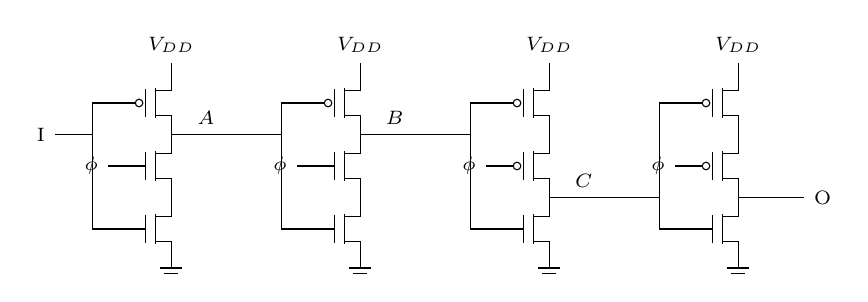
\begin{tikzpicture}[scale=.8,font=\scriptsize]
\mos{0}{4}{\phantom{I}}{1}\rail{0.25}{4.5}{V_{DD}}\mos{0}{3}{\phi}{0}\mos{0}{2}{\phantom{I}}{0}\ground{0.25}{1.5}
\node[above]at(0.8,3.5){$ A $};
\draw(-1,2)--(-1,4)--(-.75,4);\draw(-1,2)--(-.75,2);\draw(-1.6,3.5)node[left]{I}--(-1,3.5);
\mos{3}{4}{\phantom{A}}{1}\rail{3.25}{4.5}{V_{DD}}\mos{3}{3}{\phi}{0}\mos{3}{2}{\phantom{A}}{0}\ground{3.25}{1.5}
\node[above]at(3.8,3.5){$ B $};
\draw(0.25,3.5)--(2,3.5)--(2,4)--(2.25,4);\draw(2,3.5)--(2,2)--(2.25,2);
\mos{6}{4}{\phantom{B}}{1}\rail{6.25}{4.5}{V_{DD}}\mos{6}{3}{\phi}{1}\mos{6}{2}{\phantom{B}}{0}\ground{6.25}{1.5}
\node[above]at(6.8,2.5){$C$};
\draw(3.25,3.5)--(5,3.5)--(5,4)--(5.25,4);\draw(5,3.5)--(5,2)--(5.25,2);
\mos{9}{4}{\phantom{C}}{1}\rail{9.25}{4.5}{V_{DD}}\mos{9}{3}{\phi}{1}\mos{9}{2}{\phantom{C}}{0}\ground{9.25}{1.5}
\draw(6.25,2.5)--(8,2.5)--(8,4)--(8.25,4);\draw(8,2.5)--(8,2)--(8.25,2);
\draw(9.25,2.5)--(10.3,2.5)node[right]{O};\end{tikzpicture}\\Figure 4: A CMOS circuit.\end{center}
\textbf{7. (10\%)} Figure 5 shows a pipelined sequential circuit. Combinational propagation delay is 15 ns. Clock-to-Q delay, setup time, and hold time of R1/R2 are 2 ns, 3 ns, 1 ns, respectively. Determine the CLK period for the highest operation speed.
\begin{center}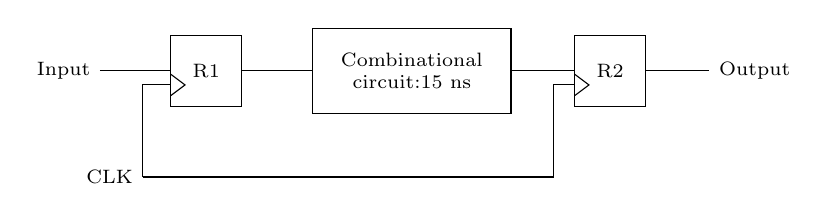
\begin{tikzpicture}[x=.9cm,y=.9cm,font=\scriptsize]
\draw(0,1.5)rectangle(1,2.5);\node at(.5,2){R1};\draw(0,1.65)--(.2,1.8)--(0,1.95);\draw(-1,2)node[left]{Input}--(0,2);\draw(1,2)--(2,2);\draw(2,1.4)rectangle(4.8,2.6);\node[align=center]at(3.4,2){Combinational\\circuit:15 ns};\draw(4.8,2)--(5.7,2);\draw(5.7,1.5)rectangle(6.7,2.5);\node at(6.2,2){R2};\draw(5.7,1.65)--(5.9,1.8)--(5.7,1.95);\draw(6.7,2)--(7.6,2)node[right]{Output};\draw(-.4,.5)node[left]{CLK}--(5.4,.5);\draw(-.4,.5)--(-.4,1.8)--(0,1.8);\draw(5.4,.5)--(5.4,1.8)--(5.7,1.8);\end{tikzpicture}\\Figure 5: A pipelined circuit.\end{center}
\small Archive note: This editable reconstruction covers the dated Fall 2007 paper. The printed percentages total 105\%; none is rescaled. Source annotations are distinguished from original printed circuit connections. All restored diagrams are editable vectors.\end{document}
